\documentclass[11pt]{article}
\usepackage[margin=1in]{geometry}
\usepackage{graphicx}
\usepackage{booktabs}
\usepackage{hyperref}
\usepackage{xcolor}
\hypersetup{colorlinks=true,linkcolor=blue,urlcolor=blue}
\title{Conservative Bid/Ask TP2 Subset Report}
\author{TP2 SPY Call Pipeline}
\date{June 2026}
\begin{document}
\maketitle

\section*{Purpose}
This report documents the conservative bid/ask TP2 subset used before the
episode-level strategy labels and rolling ML model. The broad detector uses
mid-prices to identify candidate TP2 violations. The conservative subset keeps
only rows where the violation survives immediate bid/ask execution:
\[
 A_{\mathrm{ask}}B_{\mathrm{ask}} < C_{\mathrm{bid}}D_{\mathrm{bid}}.
\]
This does not prove risk-free arbitrage, but it removes many observations where
the apparent TP2 violation exists only inside the bid/ask spread.

\section*{Construction}
\begin{itemize}
  \item Input: episode-start TP2 labels from the full Archive-2 SPY call sample.
  \item Unit: one pair episode start, not repeated daily violation rows.
  \item Active strategies after this step: T1, T2, K1, and K2.
  \item \texttt{full4} is not part of the active pipeline.
\end{itemize}

\section*{Key Accounting}
\begin{center}
\begin{tabular}{lr}
\toprule
Metric & Value \\
\midrule
Full episode-start rows & 2,098,213 \\
Conservative bid/ask TP2 rows & 228,241 \\
Kept share & 10.88\% \\
Strategy rows after removing full4 & 912,964 \\
Valid mini-backtest rows & 427,924 \\
Valid net P\&L & \$1.17B \\
Median valid return & -1.05\% \\
\bottomrule
\end{tabular}
\end{center}

\section*{Year-Level Accounting}
\begin{figure}[h]
\centering
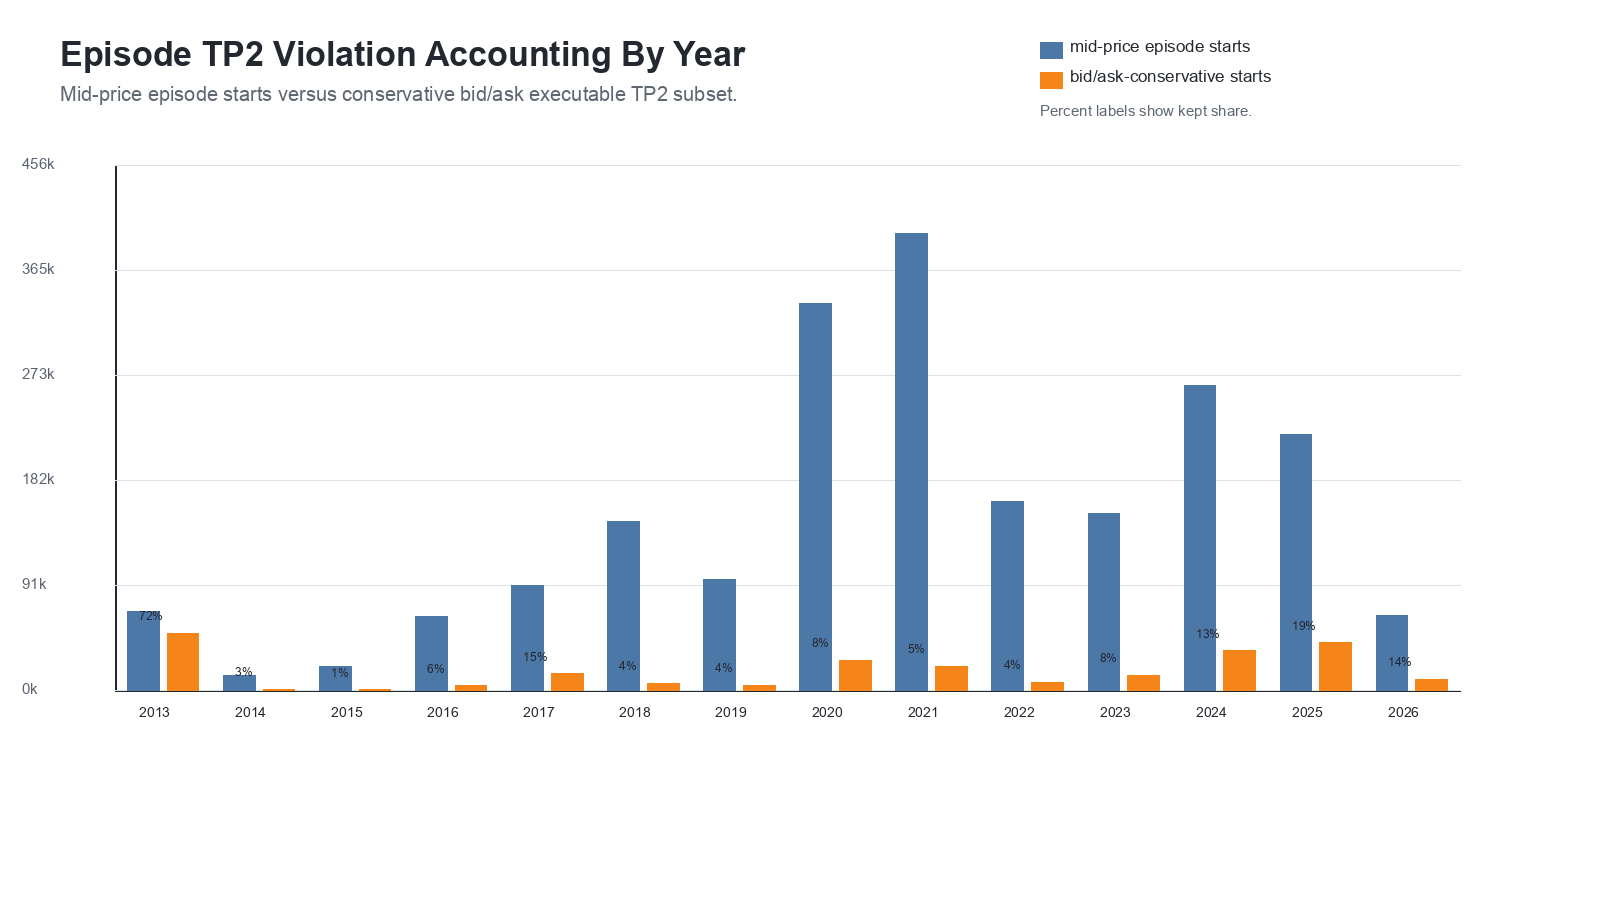
\includegraphics[width=\linewidth]{figures/mid_vs_bidask_episode_accounting_by_year.png}
\caption{Mid-detected episode starts compared with conservative bid/ask starts by year.}
\end{figure}

\section*{Interpretation}
The conservative filter is strict: only about one-tenth of mid-detected
episode starts survive. This is expected because many options, especially far
OTM rows, have wide relative spreads. The kept subset is more defensible for
trading labels, but aggregate profitability remains tail-driven, so subsequent
ML and stress tests must report hit rate, median return, and tail dependence.

\end{document}
